\chapter{Domain Model}
\label{chap:domainmodel}
Das Domain Model wurde während der Entwicklung mehrfach angepasst. In Abbildung \ref{fig:domainmodel} ist die erste und ursprüngliche Version zu sehen. In Abbildung \ref{fig:domainmodel2} ist die schliesslich umgesetzte Version zu betrachten.


\begin{figure}[h]
	\centering
	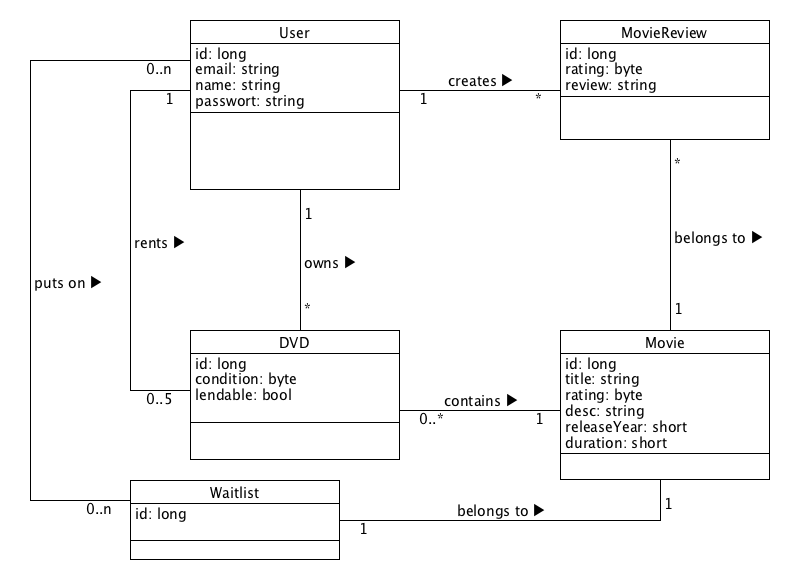
\includegraphics[width=1\textwidth]{img/domain_model.png}
	\caption{Erste Version des Domain Models}
		\label{fig:domainmodel}
\end{figure}

\section{Entitäten}

\minisec{User}
Beschreibt einen Benutzer des Systems. Er besitzt einen Namen, E-Mail Adresse und ein Passwort. Ausserdem kann er Besitzer (\emph{owns}) von mehreren \textbf{DVD}s sein. Zudem kann ein User bis zu 5 DVDs ausgeliehen haben (\textbf{RentRecord} pro Ausleihe). Weiter kann ein User einen Anspruch auf einen Film erheben, falls gerade kein DVD \enquote{frei} ist. Dann entsteht ein \textbf{ReservationRecord}. Schliesslich kann ein User Beurteilungen über Film erfassen, welche dann als \textbf{MovieReview} modelliert sind.

\minisec{DVD}
Stellt ein Model eines DVDs dar, mit einem Zustand (\emph{condition}), welcher aussagt, wie gut die DVD erhalten ist (neu, verkratzt, etc). Schliesslich kann noch erfasst werden, ob der DVD verleihbar ist (\emph{lendable}). Ein DVD lässt sich jeweils einem Film zuordnen.

\minisec{Movie}
Diese Entity stellt einen Film dar und besitzt Attribute für Titel, Länge, Rating (FSK, PEGI), Veröffentlichungsjahr und Beschreibung. Ein Movie besitzt Beurteilungen von Usern (\textbf{MovieReview}) und es kann von einem Movie mehrere \textbf{DVD}s geben. Ausserdem besitzt jeder Movie \textbf{ReservationRecords}) für alle User, die auf den Film warten, um eine DVD davon auszuleihen.

\minisec{MovieReview}
Wird von Usern zu einem bestimmten Film erstellt, besitzt ein \emph{Rating} von 1 - 10, wie gut dem User der Film gefallen hat sowie ein kurzes \emph{Review}, wo der User einen Kommentar verfassen kann.

\minisec{RentRecord}
Stellt eine Zwischen-Entität dar, die abbildet, welcher User welchen \textbf{DVD} ausgeliehen hat.

\minisec{ReservationRecord}
Ist ebenfalls eine Zwischen-Entität, die darstellt, welcher User auf welchen Film wartet, bzw. für welchen Film er einen DVD reserviert hat.

\begin{figure}[h]
	\centering
	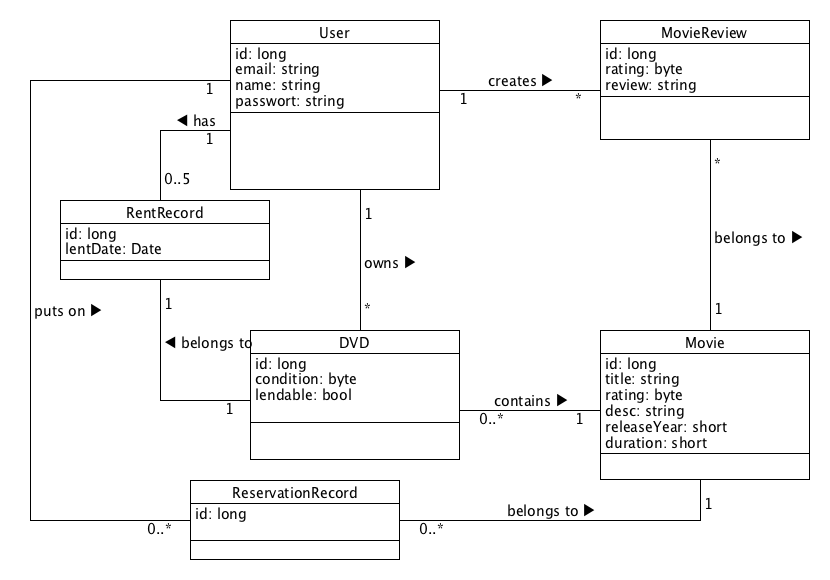
\includegraphics[width=1\textwidth]{img/domain_model2.png}
	\caption{Finale Version des Domain Models}
	\label{fig:domainmodel2}
\end{figure}

